\documentclass[aspectratio=169,10pt]{beamer}

\mode<presentation>{
  % The previous supervisor deck uses the TU Wien "Wien" theme.  Keep it when
  % available, but allow the repository to build on machines without that
  % institution-specific theme.
  \IfFileExists{beamerthemeWien.sty}
    {\usetheme[reversetitle,notitle,noauthor]{Wien}}
    {\usetheme{default}}
}

\usepackage[T1]{fontenc}
\usepackage{lmodern}
\usepackage{url}
\usepackage{graphicx}
\graphicspath{{./}{./Figures/}{./results/}}
\usepackage{appendixnumberbeamer}
\usepackage{amsmath}
\usepackage{amssymb}
\usepackage{booktabs}
\usepackage{array}
\usepackage{xcolor}
\usepackage{tikz}
\usetikzlibrary{arrows.meta,positioning,shapes.geometric}

\pdfstringdefDisableCommands{%
  \def\translate{}%
}

\definecolor{tuwred}{RGB}{140,0,0}
\definecolor{darkgreen}{RGB}{0,120,60}
\definecolor{darkblue}{RGB}{0,70,140}
\definecolor{darkorange}{RGB}{190,100,0}
\definecolor{softgray}{RGB}{245,245,245}
\definecolor{midgray}{RGB}{100,100,100}

\setbeamercolor{structure}{fg=tuwred}
\setbeamercolor{alerted text}{fg=tuwred}
\setbeamercolor{frametitle}{fg=white,bg=tuwred}
\setbeamerfont{frametitle}{series=\bfseries}
\setbeamercolor{title}{fg=tuwred}
\setbeamertemplate{navigation symbols}{}
\setbeamertemplate{footline}{%
  \hfill\usebeamerfont{page number in head/foot}%
  \color{midgray}\insertframenumber/\inserttotalframenumber\hspace{0.25cm}\vspace{0.12cm}}

\newcommand{\good}[1]{\textcolor{darkgreen}{\textbf{#1}}}
\newcommand{\warn}[1]{\textcolor{darkorange}{\textbf{#1}}}
\newcommand{\bad}[1]{\textcolor{tuwred}{\textbf{#1}}}
\newcommand{\src}[1]{\par\vspace{0.04cm}{\raggedleft\tiny\color{midgray}Source: #1\par}}
\newcommand{\tightitems}{\setlength{\itemsep}{0.25em}\setlength{\parskip}{0pt}}

\tikzset{
  flow/.style={draw=tuwred, rounded corners, thick, fill=white,
               align=center, minimum height=0.72cm, text width=1.75cm,
               inner sep=3pt, font=\scriptsize},
  softflow/.style={flow, draw=darkblue, fill=softgray},
  arrow/.style={-{Latex[length=2mm]}, thick, draw=midgray},
  smallbox/.style={draw=darkblue, rounded corners, fill=softgray,
                   align=center, minimum height=0.65cm, inner sep=3pt,
                   font=\scriptsize}
}

%%%%%%%%%%%%%%%%%%%%%%%%%%%%%%%%%%%%%%%%%%%%%%%%%%%%%%%%%%%%%%%%%%%%%%%%%%%%%
\title[EvoPress Progress]{Joint LLM Compression with EvoPress:\\Algorithm Extensions and Experimental Results}
\subtitle{Master Thesis --- Supervisor Progress Meeting}
\author[Kerim Halilovi\'c]{Kerim Halilovi\'c}
\institute[TU Wien]{TU Wien, Vienna, Austria}
\date{10 August 2026}

\begin{document}

% MAIN 1
\begin{frame}
  \titlepage
\end{frame}

%%%%%%%%%%%%%%%%%%%%%%%%%%%%%%%%%%%%%%%%%%%%%%%%%%%%%%%%%%%%%%%%%%%%%%%%%%%%%
% MAIN 2
\begin{frame}{What was agreed at the last meeting}
\small
\begin{columns}[T,onlytextwidth]
\begin{column}{0.48\textwidth}
\textbf{Questions to resolve}
\begin{itemize}\tightitems
  \item What algorithm does the source code actually execute?
  \item How does it differ from EvoPress Algorithm~1?
  \item Can sequential initialization exploit strong single-method solutions?
  \item Is crossover meaningful for the joint representation?
  \item Which extensions belong in the thesis story?
\end{itemize}
\end{column}
\begin{column}{0.48\textwidth}
\textbf{Work completed}
\begin{itemize}\tightitems
  \item[\good{$\checkmark$}] Source-level algorithm audit
  \item[\good{$\checkmark$}] Implementation-faithful pseudocode
  \item[\good{$\checkmark$}] Four sequential initialization modes
  \item[\good{$\checkmark$}] Matched G20 and G50 comparisons
  \item[\good{$\checkmark$}] Minimal component-crossover pilot
\end{itemize}
\end{column}
\end{columns}

\vspace{0.15cm}
\begin{block}{Meeting objective}
Consolidate the algorithmic contribution and decide where experimentation should stop and thesis writing should take priority.
\end{block}
\end{frame}

%%%%%%%%%%%%%%%%%%%%%%%%%%%%%%%%%%%%%%%%%%%%%%%%%%%%%%%%%%%%%%%%%%%%%%%%%%%%%
% MAIN 3
\begin{frame}{EvoPress Algorithm 1: a mutation-only $(1+\lambda)$ search}
\centering
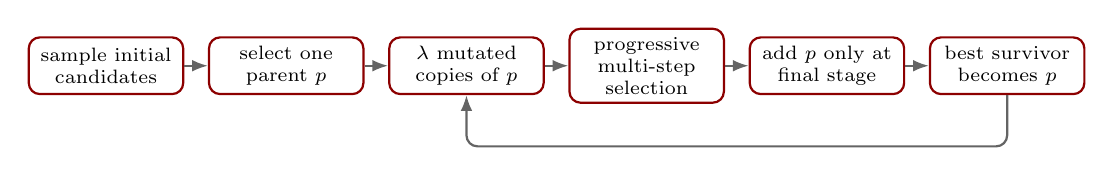
\begin{tikzpicture}[node distance=0.30cm]
  \node[flow] (init) {sample initial\\candidates};
  \node[flow, right=of init] (parent) {select one\\parent $p$};
  \node[flow, right=of parent] (mut) {$\lambda$ mutated\\copies of $p$};
  \node[flow, right=of mut] (screen) {progressive\\multi-step selection};
  \node[flow, right=of screen] (elite) {add $p$ only at\\final stage};
  \node[flow, right=of elite] (next) {best survivor\\becomes $p$};
  \draw[arrow] (init) -- (parent);
  \draw[arrow] (parent) -- (mut);
  \draw[arrow] (mut) -- (screen);
  \draw[arrow] (screen) -- (elite);
  \draw[arrow] (elite) -- (next);
  \draw[arrow, rounded corners] (next.south) -- ++(0,-0.65) -| (mut.south);
\end{tikzpicture}

\vspace{0.45cm}
\begin{columns}[T,onlytextwidth]
\begin{column}{0.48\textwidth}
\begin{block}{Level-switch mutation}
Increase one compatible unit's compression level and decrease another's, preserving the compression constraint.
\end{block}
\end{column}
\begin{column}{0.48\textwidth}
\begin{block}{Topology}
One persistent parent, local mutation, progressive screening, final-stage elitism, \bad{no crossover}.
\end{block}
\end{column}
\end{columns}
\src{EvoPress Algorithm 1; algorithm audit}
\end{frame}

%%%%%%%%%%%%%%%%%%%%%%%%%%%%%%%%%%%%%%%%%%%%%%%%%%%%%%%%%%%%%%%%%%%%%%%%%%%%%
% MAIN 4
\begin{frame}{What the official implementation actually adds}
\small
\begin{columns}[T,onlytextwidth]
\begin{column}{0.43\textwidth}
\textbf{Paper-level abstraction}
\begin{itemize}\tightitems
  \item one compression-level vector;
  \item one compatible level switch;
  \item increasingly expensive selection;
  \item final parent elitism.
\end{itemize}

\vspace{0.15cm}
\textbf{Why concise:} Algorithm~1 communicates the search principle, not every feasibility and engineering check.
\end{column}
\begin{column}{0.53\textwidth}
\textbf{Source-level behavior that matters}
\begin{itemize}\tightitems
  \item Biased switch count:
        $m=\min(U\{1,\ldots,M\},U\{1,\ldots,M\})$.
  \item Duplicate candidates are rejected.
  \item Exchanges obey group, size, and available-file restrictions.
  \item Budgets are preserved constructively; the joint extension repairs after active-set changes.
  \item The parent is inserted and re-evaluated at the final stage.
  \item Official depth search exposes population size; the default reduces to one parent.
\end{itemize}
\end{column}
\end{columns}

\vspace{0.1cm}
\begin{alertblock}{Comparison rule used in this work}
Separate the clean paper algorithm, official source behavior, and thesis-specific joint extensions.
\end{alertblock}
\src{upstream/main search implementations; ALGORITHM\_AUDIT.md, Sections 3 and 10}
\end{frame}

%%%%%%%%%%%%%%%%%%%%%%%%%%%%%%%%%%%%%%%%%%%%%%%%%%%%%%%%%%%%%%%%%%%%%%%%%%%%%
% MAIN 5
\begin{frame}{My joint candidate: depth masks plus grouped bit-widths}
\small
\begin{columns}[T,onlytextwidth]
\begin{column}{0.48\textwidth}
\centering
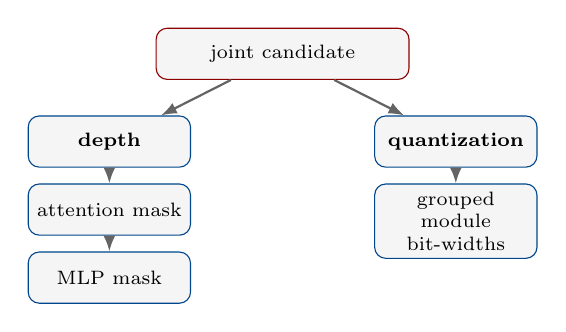
\begin{tikzpicture}[node distance=0.35cm]
  \node[smallbox, text width=3.0cm, draw=tuwred] (cand) {joint candidate};
  \node[smallbox, below left=0.45cm and -0.45cm of cand, text width=1.85cm] (depth) {\textbf{depth}};
  \node[smallbox, below right=0.45cm and -0.45cm of cand, text width=1.85cm] (quant) {\textbf{quantization}};
  \node[smallbox, below=0.2cm of depth, text width=1.85cm] (attn) {attention mask};
  \node[smallbox, below=0.2cm of attn, text width=1.85cm] (mlp) {MLP mask};
  \node[smallbox, below=0.2cm of quant, text width=1.85cm] (bits) {grouped module\\bit-widths};
  \draw[arrow] (cand) -- (depth);
  \draw[arrow] (cand) -- (quant);
  \draw[arrow] (depth) -- (attn);
  \draw[arrow] (attn) -- (mlp);
  \draw[arrow] (quant) -- (bits);
\end{tikzpicture}

\vspace{0.15cm}
{\scriptsize Main study: 32 Mistral \texttt{q\_proj} genes with 2/3/4-bit reconstructions.}
\end{column}
\begin{column}{0.48\textwidth}
\textbf{Two enforced constraints}
\begin{enumerate}\tightitems
  \item Exact structural counts:
  \[\textstyle
    \sum_l d_l^{\mathrm{attn}}=R_{\mathrm{attn}},\quad
    \sum_l d_l^{\mathrm{mlp}}=R_{\mathrm{mlp}}.
  \]
  \item Exact active bit target per compatible group:
  \[\textstyle
    |A_g(D)|^{-1}\sum_{i\in A_g(D)} b_i=B_{\mathrm{target}}.
  \]
\end{enumerate}

\begin{block}{Stored genotype versus active phenotype}
Genes inside dropped components remain stored, but do not contribute to active cost or the forward pass.
\end{block}
\end{column}
\end{columns}
\src{Algorithm audit, Sections 5--6; recorded Mistral q\_proj artifacts}
\end{frame}

%%%%%%%%%%%%%%%%%%%%%%%%%%%%%%%%%%%%%%%%%%%%%%%%%%%%%%%%%%%%%%%%%%%%%%%%%%%%%
% MAIN 6
\begin{frame}{Baseline joint search: implementation-faithful view}
\small
\begin{columns}[T,onlytextwidth]
\begin{column}{0.52\textwidth}
\begin{block}{Initialization}
Generate joint candidates, repair active budgets if needed, evaluate on \texttt{initial\_tokens}, retain one parent.
\end{block}

\begin{block}{Generate each child}
\texttt{child $\leftarrow$ deepcopy(parent)}
\begin{itemize}\tightitems
  \item with probability 0.5: depth swap(s) $\rightarrow$ active-budget repair;
  \item otherwise: active compatible quant level switch(es);
  \item reject no-op or duplicate candidates.
\end{itemize}
\end{block}
\end{column}
\begin{column}{0.44\textwidth}
\begin{block}{Progressive selection}
For each token/survivor stage:
\begin{itemize}\tightitems
  \item evaluate all remaining children on one shared minibatch;
  \item keep the best $K$;
  \item add the parent only for the final expensive stage.
\end{itemize}
The best final survivor becomes the next parent.
\end{block}

\begin{alertblock}{Legacy path preserved}
\texttt{population\_size=1} and \texttt{crossover\_probability=0} execute the established single-parent behavior.
\end{alertblock}
\end{column}
\end{columns}
\src{evo\_joint\_search.py; ALGORITHM\_AUDIT.md, Section 7}
\end{frame}

%%%%%%%%%%%%%%%%%%%%%%%%%%%%%%%%%%%%%%%%%%%%%%%%%%%%%%%%%%%%%%%%%%%%%%%%%%%%%
% MAIN 7
\begin{frame}{Main differences from EvoPress Algorithm 1}
\scriptsize
\centering
\begin{tabular}{>{\bfseries\raggedright\arraybackslash}p{2.25cm}%
                >{\raggedright\arraybackslash}p{4.55cm}%
                >{\raggedright\arraybackslash}p{5.85cm}}
\toprule
Component & EvoPress Algorithm 1 & Current joint implementation \tabularnewline
\midrule
Representation & One vector of compression levels & Attention/MLP masks plus grouped per-module bit-widths \tabularnewline
Search space & One compression allocation problem & Product space: structural depth $\times$ quantization \tabularnewline
Mutation & Compatible level switch & Mixed depth/quant mutation; optional coordinated interaction-aware mutation \tabularnewline
Constraints & One fixed compression budget & Exact depth counts plus exact active bit target per size-compatible group \tabularnewline
Inactive genes & Not central to the abstraction & Stored in the genotype; excluded from active cost when their component is dropped \tabularnewline
Feasibility & Preserved directly by compatible switches & Preserved directly where possible; repaired after depth changes alter the active set \tabularnewline
Extensions & Mutation-only $(1+\lambda)$ scaffold & Sequential warm/frozen modes and optional population crossover; replay attribution remains analysis, not search \tabularnewline
\bottomrule
\end{tabular}

\vspace{0.35cm}
\begin{block}{What remains unchanged in the baseline}
Deep-copied offspring, progressive selection, shared-stage fitness evaluation, duplicate rejection, and final-stage elitism.
\end{block}
\src{Algorithm audit; sequential and crossover implementation notes}
\end{frame}

%%%%%%%%%%%%%%%%%%%%%%%%%%%%%%%%%%%%%%%%%%%%%%%%%%%%%%%%%%%%%%%%%%%%%%%%%%%%%
% MAIN 8
\begin{frame}{Interaction-aware mutation coordinates both components}
\small
\begin{columns}[T,onlytextwidth]
\begin{column}{0.58\textwidth}
\centering
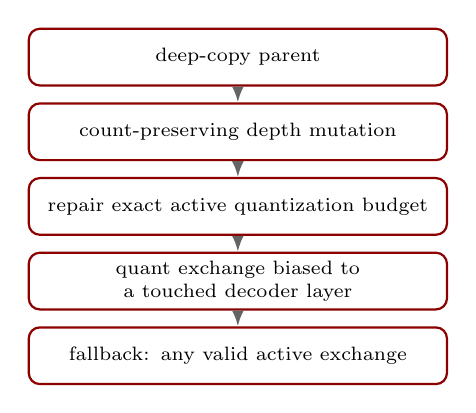
\begin{tikzpicture}[node distance=0.20cm]
  \node[flow, text width=5.1cm] (p) {deep-copy parent};
  \node[flow, text width=5.1cm, below=of p] (d) {count-preserving depth mutation};
  \node[flow, text width=5.1cm, below=of d] (r) {repair exact active quantization budget};
  \node[flow, text width=5.1cm, below=of r] (q) {quant exchange biased to a touched decoder layer};
  \node[flow, text width=5.1cm, below=of q] (c) {fallback: any valid active exchange};
  \draw[arrow] (p) -- (d);
  \draw[arrow] (d) -- (r);
  \draw[arrow] (r) -- (q);
  \draw[arrow] (q) -- (c);
\end{tikzpicture}
\end{column}
\begin{column}{0.38\textwidth}
\scriptsize
\textbf{Motivation}
\begin{itemize}\tightitems
  \item A depth change alters which quant genes are active.
  \item Independent proposals can miss the interaction.
  \item Every child coordinates both components.
\end{itemize}

\vspace{0.12cm}
\bad{Scope caveat.} ``Touched'' means decoder-layer scope, not the same subcomponent. In \texttt{q\_proj}-only search, an MLP change may bias attention quantization in that layer.

\vspace{0.2cm}
\textbf{Matched G50 signal.} WikiText2 PPL: \good{11.086} vs. 11.242; $\Delta=-0.156$, wins 2/3. Downstream macro accuracy: essentially tied.
\end{column}
\end{columns}
\src{docs/interaction\_aware\_joint\_mutation.md; interaction-aware q\_proj summary}
\end{frame}

%%%%%%%%%%%%%%%%%%%%%%%%%%%%%%%%%%%%%%%%%%%%%%%%%%%%%%%%%%%%%%%%%%%%%%%%%%%%%
% MAIN 9
\begin{frame}{Sequential initialization: four stage-two variants}
\small
\begin{columns}[T,onlytextwidth]
\begin{column}{0.49\textwidth}
\begin{block}{Depth $\rightarrow$ Quantization, frozen}
Import depth exactly; search only active quantization assignments.
\end{block}
\begin{block}{Depth $\rightarrow$ Joint, warm}
Import depth exactly for initialization; then allow the selected joint operator to modify both components.
\end{block}
\end{column}
\begin{column}{0.49\textwidth}
\begin{block}{Quantization $\rightarrow$ Depth, frozen}
Import quantization exactly; search only contribution-compatible depth swaps that preserve the active budget.
\end{block}
\begin{block}{Quantization $\rightarrow$ Joint, warm}
Import quantization unchanged under strict initialization; then allow ordinary joint refinement.
\end{block}
\end{column}
\end{columns}

\vspace{0.2cm}
\begin{columns}[T,onlytextwidth]
\begin{column}{0.49\textwidth}
\good{Frozen} = stage-one component is an invariant throughout stage two.
\end{column}
\begin{column}{0.49\textwidth}
\warn{Warm} = stage-one component fixes the start, not the final candidate.
\end{column}
\end{columns}

\vspace{0.2cm}
\begin{alertblock}{Why quantization-first frozen is special}
Without repair, a depth swap is legal only when removed and restored components have equal bit-sum and module-count contribution vectors in every group.
\end{alertblock}
\src{SEQUENTIAL\_SEARCH\_IMPLEMENTATION.md}
\end{frame}

%%%%%%%%%%%%%%%%%%%%%%%%%%%%%%%%%%%%%%%%%%%%%%%%%%%%%%%%%%%%%%%%%%%%%%%%%%%%%
% MAIN 10
\begin{frame}{Sequential results: direction and operator both matter}
\centering
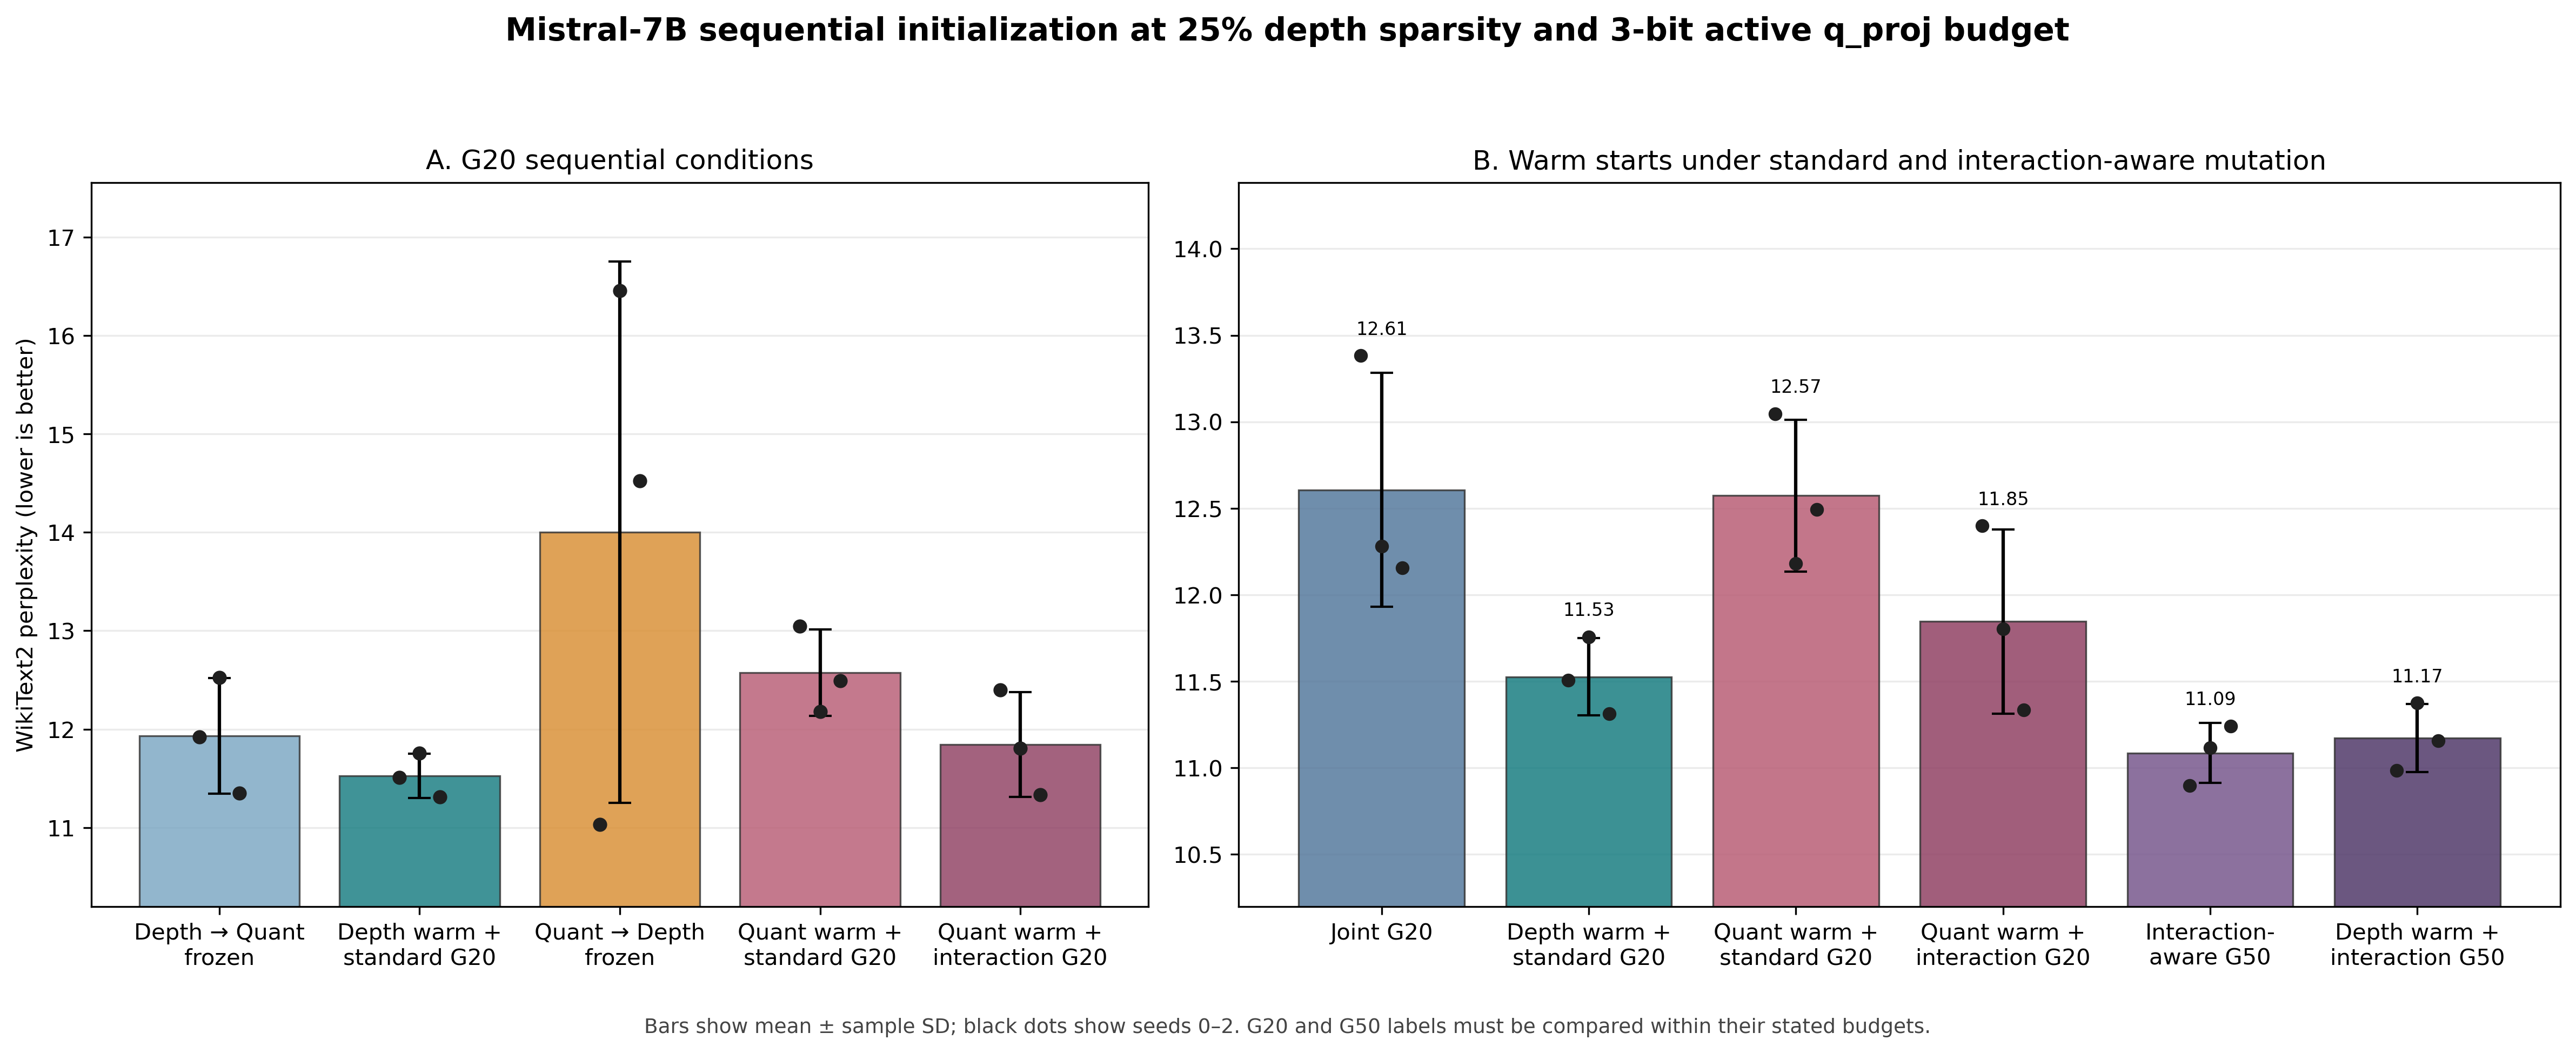
\includegraphics[width=0.98\textwidth,height=0.75\textheight,keepaspectratio]{sequential_search_comparison.png}

\vspace{-0.15cm}
{\scriptsize Bars show mean $\pm$ sample SD; dots are seeds 0--2. Compare G20 and G50 only within their stated budgets.}
\src{results/sequential\_search\_comparison.png and .md}
\end{frame}

%%%%%%%%%%%%%%%%%%%%%%%%%%%%%%%%%%%%%%%%%%%%%%%%%%%%%%%%%%%%%%%%%%%%%%%%%%%%%
% MAIN 11
\begin{frame}{What sequential initialization tells us}
\small
\begin{columns}[T,onlytextwidth]
\begin{column}{0.48\textwidth}
\textbf{G20 observations}
\begin{itemize}\tightitems
  \item \good{Depth warm + standard: $11.526\pm0.223$} --- best G20 sequential condition.
  \item Depth frozen + quant search: $11.932\pm0.586$ --- little gain beyond composition.
  \item Quant $\rightarrow$ depth frozen: $14.003\pm2.748$ --- highly seed-variable.
  \item Quant warm + standard: $12.573\pm0.439$; interaction-aware: \good{$11.846\pm0.532$}.
\end{itemize}
\end{column}
\begin{column}{0.48\textwidth}
\textbf{Matched paired deltas (method minus baseline)}
\tiny
\begin{tabular}{p{3.25cm}rr}
\toprule
Comparison & $\Delta$ PPL & Wins \\
\midrule
Quant warm IA $-$ quant warm standard & $-0.727\pm0.396$ & 3/3 \\
Quant warm IA $-$ standard-init IA & $-0.286\pm0.918$ & 2/3 \\
Standard-init IA $-$ standard-init standard & $-0.474\pm1.128$ & 2/3 \\
\bottomrule
\end{tabular}

\vspace{0.2cm}
\begin{alertblock}{Evidence boundary}
Three paired seeds: descriptive evidence, not a statistical-significance claim.
\end{alertblock}
\end{column}
\end{columns}

\vspace{0.1cm}
\textbf{Interpretation:} initialization is direction-dependent, and its value depends on the stage-two mutation operator.
\src{results/sequential\_search\_comparison.md; paired deltas CSV}
\end{frame}

%%%%%%%%%%%%%%%%%%%%%%%%%%%%%%%%%%%%%%%%%%%%%%%%%%%%%%%%%%%%%%%%%%%%%%%%%%%%%
% MAIN 12
\begin{frame}{Warm start versus a longer search}
\centering
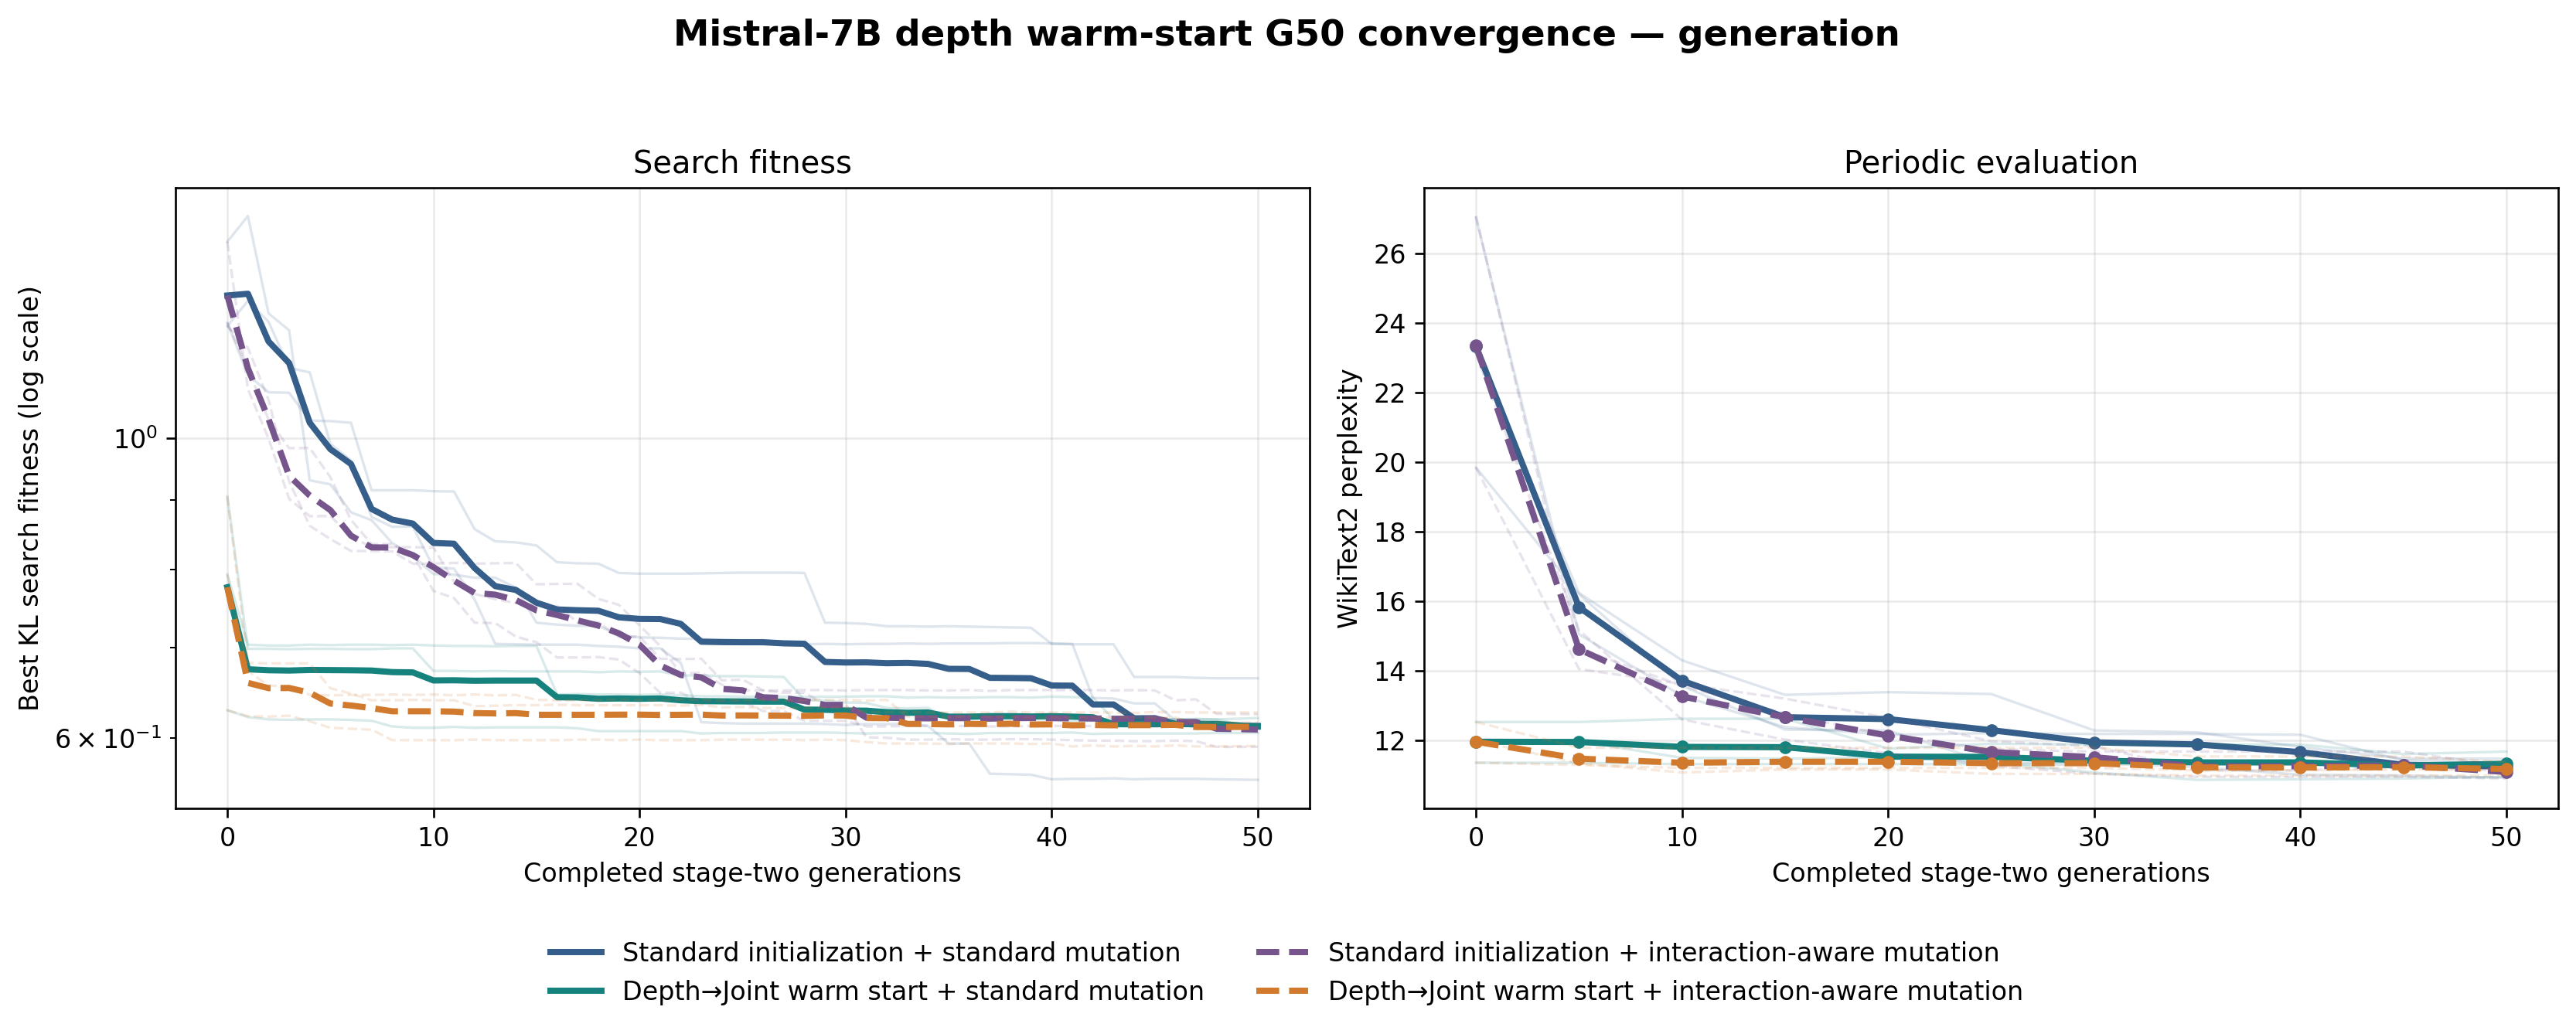
\includegraphics[width=0.90\textwidth,height=0.52\textheight,keepaspectratio]{depth_warmstart_g50_convergence_generation.png}

\vspace{-0.05cm}
\begin{columns}[T,onlytextwidth]
\begin{column}{0.48\textwidth}
\textbf{Early / moderate budget}\par
Warm starts begin much stronger and retain an advantage around generation 20.
\end{column}
\begin{column}{0.48\textwidth}
\textbf{Matched interaction-aware G50}\par
Depth warm $-$ standard init: \warn{$+0.086\pm0.172$ PPL}, wins 1/3.
\end{column}
\end{columns}

\vspace{0.12cm}
\centering\small\textbf{Conclusion:} warm starting mainly changes convergence speed and early quality, not the final G50 basin.
\src{results/depth\_warmstart\_g50\_comparison.md and convergence figure}
\end{frame}

%%%%%%%%%%%%%%%%%%%%%%%%%%%%%%%%%%%%%%%%%%%%%%%%%%%%%%%%%%%%%%%%%%%%%%%%%%%%%
% MAIN 13
\begin{frame}{Why investigate crossover?}
\begin{columns}[T,onlytextwidth]
\begin{column}{0.49\textwidth}
\textbf{Ordinary population GA}
\begin{center}
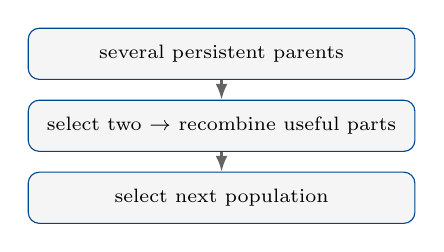
\begin{tikzpicture}[node distance=0.25cm]
  \node[smallbox, text width=4.7cm] (pop) {several persistent parents};
  \node[smallbox, text width=4.7cm, below=of pop] (cross) {select two $\rightarrow$ recombine useful parts};
  \node[smallbox, text width=4.7cm, below=of cross] (surv) {select next population};
  \draw[arrow] (pop)--(cross); \draw[arrow] (cross)--(surv);
\end{tikzpicture}
\end{center}
\end{column}
\begin{column}{0.49\textwidth}
\textbf{EvoPress baseline}
\begin{center}
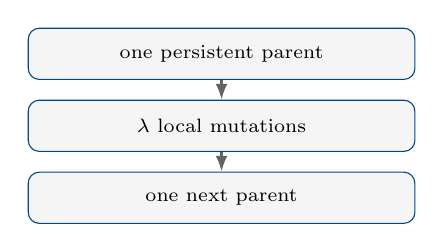
\begin{tikzpicture}[node distance=0.25cm]
  \node[smallbox, text width=4.7cm] (p) {one persistent parent};
  \node[smallbox, text width=4.7cm, below=of p] (m) {$\lambda$ local mutations};
  \node[smallbox, text width=4.7cm, below=of m] (n) {one next parent};
  \draw[arrow] (p)--(m); \draw[arrow] (m)--(n);
\end{tikzpicture}
\end{center}
\end{column}
\end{columns}

\vspace{0.3cm}
\begin{block}{Motivation for this joint search}
The candidate already factorizes into depth and quantization. If different persistent candidates contain useful components, recombination may combine them more directly than repeated local mutation.
\end{block}

\begin{alertblock}{Necessary algorithmic change}
Crossover is not meaningful with only one persistent parent; a small population must first be retained.
\end{alertblock}
\end{frame}

%%%%%%%%%%%%%%%%%%%%%%%%%%%%%%%%%%%%%%%%%%%%%%%%%%%%%%%%%%%%%%%%%%%%%%%%%%%%%
% MAIN 14
\begin{frame}{Minimal component crossover}
\small
\begin{columns}[T,onlytextwidth]
\begin{column}{0.47\textwidth}
\begin{align*}
 A &= (D_A,Q_A), & B &= (D_B,Q_B),\\
 C_1 &= (\textcolor{darkgreen}{D_A},\textcolor{darkblue}{Q_B}), &
 C_2 &= (\textcolor{darkgreen}{D_B},\textcolor{darkblue}{Q_A}).
\end{align*}

\centering
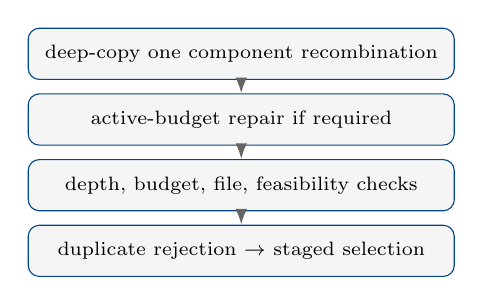
\begin{tikzpicture}[node distance=0.17cm]
  \node[smallbox, text width=5.2cm] (rec) {deep-copy one component recombination};
  \node[smallbox, text width=5.2cm, below=of rec] (rep) {active-budget repair if required};
  \node[smallbox, text width=5.2cm, below=of rep] (valid) {depth, budget, file, feasibility checks};
  \node[smallbox, text width=5.2cm, below=of valid] (dup) {duplicate rejection $\rightarrow$ staged selection};
  \draw[arrow] (rec)--(rep); \draw[arrow] (rep)--(valid); \draw[arrow] (valid)--(dup);
\end{tikzpicture}
\end{column}
\begin{column}{0.49\textwidth}
\textbf{Pilot configuration}
\begin{itemize}\tightitems
  \item population 4; crossover probability 0.25;
  \item distinct parents, selected uniformly;
  \item otherwise unchanged standard mutation;
  \item configured schedule $[8,2,1]$;
  \item effective schedule $[8,2,4]$;
  \item all parents join final-stage elitism.
\end{itemize}

\vspace{0.15cm}
\bad{Repair semantics.} If repair changes $Q$, report \emph{component crossover + repair}.
\end{column}
\end{columns}
\src{CROSSOVER\_IMPLEMENTATION.md; component-crossover tests}
\end{frame}

%%%%%%%%%%%%%%%%%%%%%%%%%%%%%%%%%%%%%%%%%%%%%%%%%%%%%%%%%%%%%%%%%%%%%%%%%%%%%
% MAIN 15
\begin{frame}{Crossover result: feasible, but little useful novelty}
\small
\begin{columns}[T,onlytextwidth]
\begin{column}{0.56\textwidth}
\small
\begin{tabular}{lrr}
\toprule
 & Component crossover & Mutation-only \\
\midrule
PPL & $12.870\pm0.927$ & $12.607\pm0.675$ \\
KL & $0.779\pm0.061$ & $0.735\pm0.051$ \\
Runtime & $694\pm51$ s & $609\pm2$ s \\
\bottomrule
\end{tabular}

\vspace{0.35cm}
\begin{itemize}\tightitems
  \item PPL better for 2/3 seeds, but mean worse.
  \item KL mixed and mean worse.
  \item Mean runtime increased by approximately 14\%.
\end{itemize}
\end{column}
\begin{column}{0.40\textwidth}
\begin{block}{Proposal diagnostics}
\begin{itemize}\tightitems
  \item attempted: 301;
  \item accepted: 63 (20.9\%);
  \item \bad{duplicates: 238 (79.1\%)};
  \item infeasible: 0;
  \item accepted with repair: 25/63;
  \item population diversity: 4/4 every generation.
\end{itemize}
\end{block}
\end{column}
\end{columns}

\vspace{0.12cm}
\textbf{Interpretation:} technically feasible, but the population provides too few distinct depth/quant combinations to add much diversity.

\vspace{0.12cm}
\begin{alertblock}{Causal limitation}
Population changed $1\rightarrow4$ and crossover probability $0\rightarrow0.25$: this tests the full extension, not crossover alone.
\end{alertblock}
\src{CROSSOVER\_EXPERIMENT\_HANDOFF.md; committed run summaries}
\end{frame}

%%%%%%%%%%%%%%%%%%%%%%%%%%%%%%%%%%%%%%%%%%%%%%%%%%%%%%%%%%%%%%%%%%%%%%%%%%%%%
% MAIN 16
\begin{frame}{Current conclusions and next steps}
\small
\begin{columns}[T,onlytextwidth]
\begin{column}{0.49\textwidth}
\textbf{Current algorithmic story}
\begin{itemize}\tightitems
  \item EvoPress remains an effective scaffold for joint compression.
  \item Interaction-aware mutation is the most promising operator extension.
  \item Sequential initialization can improve early search, but depends on direction and operator.
  \item Component crossover is feasible, but did not improve this setting and generated many duplicates.
  \item Replay attribution explains outcomes; it is analysis, not search.
\end{itemize}
\end{column}
\begin{column}{0.49\textwidth}
\textbf{Recommended priority}
\begin{enumerate}\tightitems
  \item Freeze the method and formal algorithm.
  \item Convert the audit into the methodology chapter.
  \item Select final tables, plots, and cost conventions.
  \item Decide whether one scoped attention/downstream evaluation is necessary.
  \item Prioritize writing over more operators.
\end{enumerate}
\end{column}
\end{columns}

\vspace{0.15cm}
\begin{alertblock}{Proposed decision}
The algorithmic contribution is sufficiently developed; remaining experiments should close specific evidence gaps, not expand the operator catalog.
\end{alertblock}
\end{frame}

%%%%%%%%%%%%%%%%%%%%%%%%%%%%%%%%%%%%%%%%%%%%%%%%%%%%%%%%%%%%%%%%%%%%%%%%%%%%%
\appendix

% BACKUP 1 / SLIDE 17
\begin{frame}{Backup: full current search pseudocode}
\scriptsize
\begin{columns}[T,onlytextwidth]
\begin{column}{0.49\textwidth}
\begin{block}{Initialization}
\ttfamily
validate configuration\\
$C_0 \leftarrow$ feasible initial candidates\\
$P \leftarrow$ select best population\_size from $C_0$\\
assert unique($P$)
\end{block}

\begin{block}{Offspring generation}
\ttfamily
while $|O| < \lambda$:\\
\quad if crossover enabled and sample():\\
\qquad $a,b\leftarrow$ distinct uniform parents\\
\qquad $c\leftarrow$ component\_crossover($a,b$)\\
\qquad repair active budget if required\\
\quad else:\\
\qquad $a\leftarrow$ uniform parent\\
\qquad $c\leftarrow$ selected existing mutation($a$)\\
\quad reject infeasible/no-op/duplicate $c$\\
\quad $O\leftarrow O\cup\{c\}$
\end{block}
\end{column}
\begin{column}{0.49\textwidth}
\begin{block}{Selection and reporting}
\ttfamily
for each intermediate $(K,T)$:\\
\quad $O\leftarrow$ best $K$ on $T$ tokens\\[0.15cm]
$O\leftarrow O\cup P$ \quad // final elitism\\
$P\leftarrow$ best population\_size unique candidates\\
fail if $|P|<$ population\_size\\
report best member of $P$\\
repeat for next generation
\end{block}

\begin{alertblock}{Reduction to the baseline}
With population size 1 and crossover probability 0, this reduces to the legacy $(1+\lambda)$ joint search without consuming new parent-selection randomness.
\end{alertblock}
\end{column}
\end{columns}
\end{frame}

%%%%%%%%%%%%%%%%%%%%%%%%%%%%%%%%%%%%%%%%%%%%%%%%%%%%%%%%%%%%%%%%%%%%%%%%%%%%%
% BACKUP 2 / SLIDE 18
\begin{frame}{Backup: active-budget repair}
\small
For quantization group $g$, depth state $D$, active set $A_g(D)$, and target $B$:
\[
 C_g(D,Q)=\sum_{i\in A_g(D)} b_i,
 \qquad C_g(D,Q)=|A_g(D)|B.
\]

\begin{columns}[T,onlytextwidth]
\begin{column}{0.48\textwidth}
\textbf{Why repair is needed}
\begin{itemize}\tightitems
  \item A depth swap changes $A_g(D)$.
  \item The imported/stored $Q$ may then violate the exact target.
  \item A crossover child can combine a quant profile optimized under a different depth mask.
\end{itemize}
\end{column}
\begin{column}{0.48\textwidth}
\textbf{What repair does}
\begin{itemize}\tightitems
  \item Preserve the selected depth mask exactly.
  \item Increment/decrement available active bit levels within size-compatible groups.
  \item Stop only at the exact integer target sum; otherwise reject/fail clearly.
  \item Record how many quant genes changed.
\end{itemize}
\end{column}
\end{columns}

\vspace{0.3cm}
\begin{alertblock}{q\_proj scope detail}
Dropping attention deactivates its \texttt{q\_proj}; dropping only the MLP does not deactivate an attention projection in the same decoder layer.
\end{alertblock}
\end{frame}

%%%%%%%%%%%%%%%%%%%%%%%%%%%%%%%%%%%%%%%%%%%%%%%%%%%%%%%%%%%%%%%%%%%%%%%%%%%%%
% BACKUP 3 / SLIDE 19
\begin{frame}{Backup: full sequential quality table}
\scriptsize
\centering
\begin{tabular}{p{7.5cm}rcc}
\toprule
Method & WikiText2 PPL & G & Role \\
\midrule
Depth + uniform 3-bit q\_proj & $11.953\pm0.586$ & -- & composition \\
Independent depth + searched q\_proj & $11.947\pm0.585$ & -- & composition \\
Standard init + standard mutation & $12.607\pm0.675$ & 20 & control \\
Standard init + interaction-aware & $12.133\pm0.508$ & 20 & control \\
Depth $\rightarrow$ quantization, frozen & $11.932\pm0.586$ & 20 & sequential \\
Depth $\rightarrow$ joint warm + standard & \good{$11.526\pm0.223$} & 20 & sequential \\
Quantization $\rightarrow$ depth, frozen & $14.003\pm2.748$ & 20 & sequential \\
Quantization $\rightarrow$ joint warm + standard & $12.573\pm0.439$ & 20 & sequential \\
Quantization $\rightarrow$ joint warm + interaction-aware & $11.846\pm0.532$ & 20 & sequential \\
Standard joint & $11.242\pm0.285$ & 50 & reference \\
Interaction-aware joint & \good{$11.086\pm0.174$} & 50 & reference \\
Depth warm + interaction-aware & $11.172\pm0.196$ & 50 & reference \\
\bottomrule
\end{tabular}

\vspace{0.25cm}
{\small G50 rows are longer-search references and are not pooled with the G20 comparison. Values are mean $\pm$ sample SD over seeds 0--2.}
\end{frame}

%%%%%%%%%%%%%%%%%%%%%%%%%%%%%%%%%%%%%%%%%%%%%%%%%%%%%%%%%%%%%%%%%%%%%%%%%%%%%
% BACKUP 4 / SLIDE 20
\begin{frame}{Backup: sequential cost accounting}
\tiny
\centering
\begin{tabular}{p{4.75cm}rrrrr}
\toprule
Method & Stage 1 & Stage 2 & E2E & Stage-2 evals & E2E evals \\
 & min & min & min & & \\
\midrule
Standard init + standard G20 & 0.00 & 10.15 & 10.15 & 572 & 572 \\
Standard init + interaction-aware G20 & 0.00 & 9.54 & 9.54 & 572 & 572 \\
Quant warm + standard G20 & 13.15 & 9.01 & 22.16 & 572 & 1,144 \\
Quant warm + interaction-aware G20 & 13.15 & 11.39 & 24.54 & 572 & 1,144 \\
\bottomrule
\end{tabular}

\vspace{0.35cm}
\begin{columns}[T,onlytextwidth]
\begin{column}{0.48\textwidth}
\textbf{Stage-two accounting}
\begin{itemize}\tightitems
  \item Matches generations, offspring, and selection schedule.
  \item Useful for studying initialization/operator behavior.
  \item Depth-first modes evaluate one initial stage-two candidate; quant-first and standard initialization evaluate 32.
\end{itemize}
\end{column}
\begin{column}{0.48\textwidth}
\textbf{End-to-end accounting}
\begin{itemize}\tightitems
  \item Adds the seed-matched stage-one search.
  \item Necessary for method-level compute comparisons.
  \item Runtime is approximate across restarted DataLab sessions; candidate evaluations and token exposure are more reproducible.
\end{itemize}
\end{column}
\end{columns}
\src{results/sequential\_search\_comparison.md}
\end{frame}

%%%%%%%%%%%%%%%%%%%%%%%%%%%%%%%%%%%%%%%%%%%%%%%%%%%%%%%%%%%%%%%%%%%%%%%%%%%%%
% BACKUP 5 / SLIDE 21
\begin{frame}{Backup: crossover diagnostics by seed}
\scriptsize
\centering
\begin{tabular}{rrrrrrrrr}
\toprule
Seed & Attempted & Accepted & Duplicates & Repaired & Cross PPL & Ctrl PPL & Cross KL & Ctrl KL \\
\midrule
0 & 107 & 22 & 85 & 10 & 12.664 & 13.383 & 0.772 & 0.794 \\
1 & 93  & 25 & 68 & 13 & 13.883 & 12.281 & 0.843 & 0.699 \\
2 & 101 & 16 & 85 & 2  & 12.062 & 12.156 & 0.722 & 0.713 \\
\midrule
Total/mean & 301 & 63 & 238 & 25 & 12.870 & 12.607 & 0.779 & 0.735 \\
\bottomrule
\end{tabular}

\vspace{0.35cm}
\begin{columns}[T,onlytextwidth]
\begin{column}{0.48\textwidth}
\begin{block}{Operational result}
Acceptance 20.9\%; duplicate rate 79.1\%; infeasible 0/301; repair among accepted crossover children 25/63 (39.7\%).
\end{block}
\end{column}
\begin{column}{0.48\textwidth}
\begin{block}{Quality result}
Mixed seed outcomes; no consistent improvement in PPL or KL; population remained 4/4 unique in every generation.
\end{block}
\end{column}
\end{columns}

\begin{alertblock}{Unisolated factor}
A population-four, crossover-zero control would be required to separate the effect of population size from the crossover operator.
\end{alertblock}
\end{frame}

%%%%%%%%%%%%%%%%%%%%%%%%%%%%%%%%%%%%%%%%%%%%%%%%%%%%%%%%%%%%%%%%%%%%%%%%%%%%%
% BACKUP 6 / SLIDE 22
\begin{frame}{Backup: evidence boundaries and limitations}
\small
\begin{columns}[T,onlytextwidth]
\begin{column}{0.49\textwidth}
\textbf{Experimental scope}
\begin{itemize}\tightitems
  \item Three seeds: descriptive means, SDs, and paired wins.
  \item Main evidence: Mistral-7B, WikiText2, 25\% separate attention/MLP sparsity.
  \item \texttt{q\_proj}-only scope; exact active 3-bit target.
  \item G20 and G50 use different budgets.
\end{itemize}
\end{column}
\begin{column}{0.49\textwidth}
\textbf{What is not established}
\begin{itemize}\tightitems
  \item No significance or broad generalization claim.
  \item No claim that sequential initialization always helps.
  \item No claim that crossover alone is harmful or beneficial.
  \item Compression is theoretical weight accounting, not latency or packed checkpoint size.
  \item Runtime varies across DataLab sessions.
\end{itemize}
\end{column}
\end{columns}

\vspace{0.18cm}
\begin{block}{Methodological distinction}
Replay attribution evaluates saved candidates post hoc; sequential initialization and crossover change the search itself.
\end{block}
\end{frame}

\end{document}
